% diary.sty 検証用: tikzpicture 環境が使えること、
% 図があるページでもライセンスフッターが焼き込まれることの確認
\documentclass[paper=a4]{jlreq}
\usepackage[problem]{diary}

\begin{document}
\diarytitle{0001}{放物線と直線}

放物線 $y = x^2$ と直線 $y = x + 2$ の共有点、および概形は次のとおりである。
（$x^2 = x+2$ より $x=-1,2$。calc ライブラリで交点座標を計算して描画する。）

\begin{center}
\begin{tikzpicture}[domain=-2.5:2.5, scale=0.9]
  \draw[->] (-2.5,0) -- (2.5,0) node[right] {$x$};
  \draw[->] (0,-1) -- (0,5) node[above] {$y$};
  \draw[thick] plot (\x, {\x*\x}) node[right] {$y=x^2$};
  \draw[thick] plot (\x, {\x+2}) node[right] {$y=x+2$};
  \coordinate (P1) at (-1,1);
  \coordinate (P2) at (2,4);
  \fill[red] (P1) circle (2pt);
  \fill[red] (P2) circle (2pt);
  \draw[dashed] (P1) -- ($(P1)+(0,-1)$);
  \draw[dashed] (P2) -- ($(P2)+(0,-1)$);
\end{tikzpicture}
\end{center}

% 全ページにフッターが焼き込まれることを検証するため、2 ページ目を追加する。
\newpage

図を用いた 2 ページ目でもフッターが表示されることを確認する。

\begin{center}
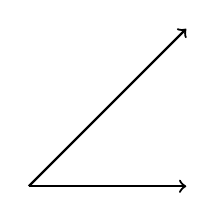
\begin{tikzpicture}
  \draw[thick, ->] (0,0) -- (2,2);
  \draw[thick, ->] (0,0) -- (2,0);
\end{tikzpicture}
\end{center}

\end{document}
